\chapter{インターネットプロトコル層(その1) インターネットプロトコルの概論}

この章では、インターネットプロトコルスイートにおける、インターネットプロトコル層について、概論的な説明をします。インターネットプロトコル層は、トランスポート層にどのようなサービスを提供するのでしょうか。そして、どのようにネットワークアクセス層を利用しているのでしょうか。

インターネットプロトコル層とは、その名の通り、複数のネットワークとネットワークの間で通信を行うためのプロトコルです。そして、TCP/IPのIPに相当するプロトコルでもあります。

何らかの機器をインターネット接続する際に、必ず、IPアドレスという言葉がでてきます。このIPとはInternet Protocolであり、略さずに言えば、Internet Protocol Addressとなります。では、インターネットプロトコルとはなにであるのか、そして、IPアドレスとは何であるのかを説明していくことにしましょう。

\section{インターネット}

インターネットとという言葉ある。そして、インターネットプロトコル層というレイヤーがある。

なぜインターネットプロトコル層が必要なのだろうか?ネットワークアクセス層の章を読み進めいていただいていたら、このような疑問を持たれるかもしれない。
そして、ネットワークアクセス層だけで世界中と通信すればいいのに、そうしない理由は何なのだろうか。

前章で説明したように、ネットワークコミュニケーション層の物理的な規格とプロトコルには、いろいろなものがある。イーサネットは狭い範囲でホストの数が多い場合に向いているし、PPPは、距離にかかわらず、一対一接続を行う場合に向いている。

それなら、ネットワークコミュニケーション層ごとに、プロトコル変換を行うものを置けばいいと思うかもしれない。だが、それなら、複数のネットワークを結ぶプロトコルを定めて、ネットワークアクセス層と、ネットワーク間のプロトコルを取り持つ機器にした方が汎用性が増すのではないだろうか。

そのような発想で、インターネットプロトコルが生まれた。インターネットという言葉は、inter-netである。つまり、ネットワークとネットワークの間、ということだ。

\subsection{インターネットプロトコル層の昔話}

ここでも、インターネットプロトコル成立前夜の状況を振り返る昔話から始めよう。規格の由来というのは、全て昔話のなかに隠れている。
後のインターネットに受け継がれる思想と技術は、1960年代後半から、アメリカの四つの大学を結ぶネットワークのARPANETからはじまった。

そんな中、ロバート・カーンは衛星パケット網と地上の無線パケット網の相互接続実験を行っていた。その過程で、カーンは、異なるネットワークの相互接続ができるということについての知見を得た。
今の用語で言えば、異なる構造のネットワークアクセス層同士の通信を行う、ということである。
現在でも、一般的なインターネット接続は、LANとインターネット接続回線という、異なる構造のネットワークアクセス層どうしの通信を行っている。
TCP/IPの原初の形は1973年から1974年頃に、RFC675としてまとめられた。ALTO ALOHAがEthernetという名前になる前後である。このころは、LANを構成するための、ネットワークコミュニケーション層相当の規格でも、ベンダーごとにまちまちな構造、規格、プロトコルであった。

\subsection{異なるネットワークの間の通信}

異なるネットワーク間で通信をするということは、それぞれの機器が直接に接続されているネットワークコミュニケーション層の規格を問わず、エンドツーエンドでデータを届けるということである。
それぞれのネットワークは、自分と、自分以外のネットワーク全てが、そのネットワークコミュニケーション層では、宛先にフレームを届けることができることを期待する。

もうひとつ、あるネットワークから来たパケットからデータを取りだして、宛先となるネットワーク宛のパケットに作り直して送る、中継の仕組みも用意しよう。
この二つで、異なるネットワークの間で、とりあえずデータを相互に送りあうことができるだろう。

では、この異なるネットワークでデータを相互に送りあうこととはどういうことか、二つのネットワークを繋ぐところから初めて、順を追って説明していこう。

\subsection{二つのネットワークを結ぶ}

\begin{figure}[htbp]
	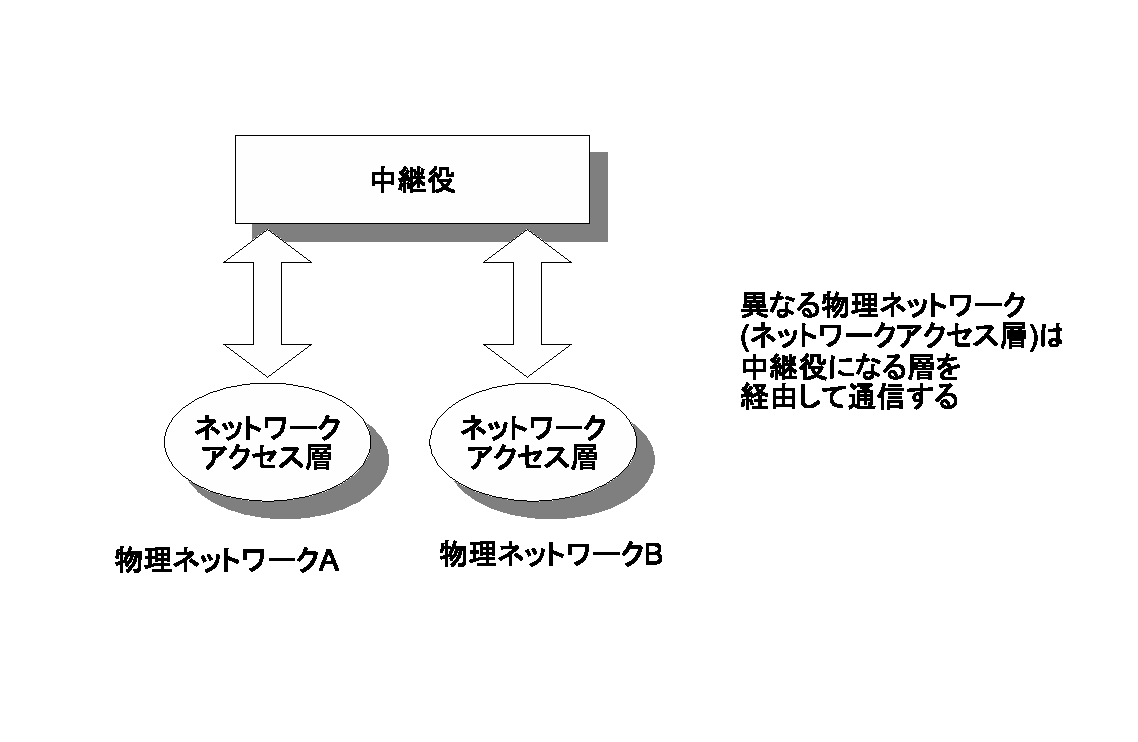
\includegraphics[width=12cm,clip]{draw/ip_basic2.eps}
	\caption{二つのネットワークを結ぶ}
	\label{fig:ip_basic2}
\end{figure}

二つのネットワークを一つの中継役が結んでいる場合で考えてみよう。中継役はネットワークAとネットワークBとに接続されたコンピュータである。そして、それぞれのネットワークに対してネットワークコミュニケーション層のプロトコルで通信することができる。
だが、ネットワークAとおネットワークBhは、ネットワークコミュニケーション層のプロトコルでは相互に通信でないとする。

ネットワークAのホストからネットワークBのホストに宛てた通信は、とりあえず中継役に送る。中継役は、ネットワークB宛の通信が届いたら、ネットワークBのネットワークコミュニケーション層のプロトコルで、宛先に通信を届ける。ネットワークBからネットワークAへの通信も同様である。

中継役を置くことで、それぞれのネットワークに属するホストが、自分の所属していない側のネットワークコミュニケーション層の情報をもっていないくても、相互に通信が可能になる。つまり、自分以外のネットワークに関して、持っていなければならない情報を減らすことができる。

一方、中継役は、中継に必要なアプリケーションのみ動作させればいい。
そのため、コンピュータとしてのリソースを中継に使うことができる。

\subsection{三つ以上のネットワークを結ぶ}

つぎに、三つ以上のネットワークを結ぶ場合を考えてみよう。三つ以上のネットワークをそれぞれ中継役で結んでやる。ここでは、簡単にするために、図\ref{fig:ip_basic3}のようにネットワークが接続されているとしよう。

ネットワークAとネットワークB、ネットワークBとネットワークCの」間の通信は、先に説明したふたつのネットワークを接続した場合となる。では、ネットワークAとネットワークCの間の通信はどうなるのであろうか。

ネットワークAの中のホストは、宛先をネットワークCのホストにした通信を、ネットワークAとネットワークBの中継役に転送する。ネットワークAとネットワークBの中継役は、宛先がCであるのを確認すると、ネットワークB二接続されている、ネットワークBとネットワークCの中継役に転送する。最終的に、ネットワークBとネットワークCの中継役が、ネットワークCに接続されたホストに中継する。


\begin{figure}[htbp]
	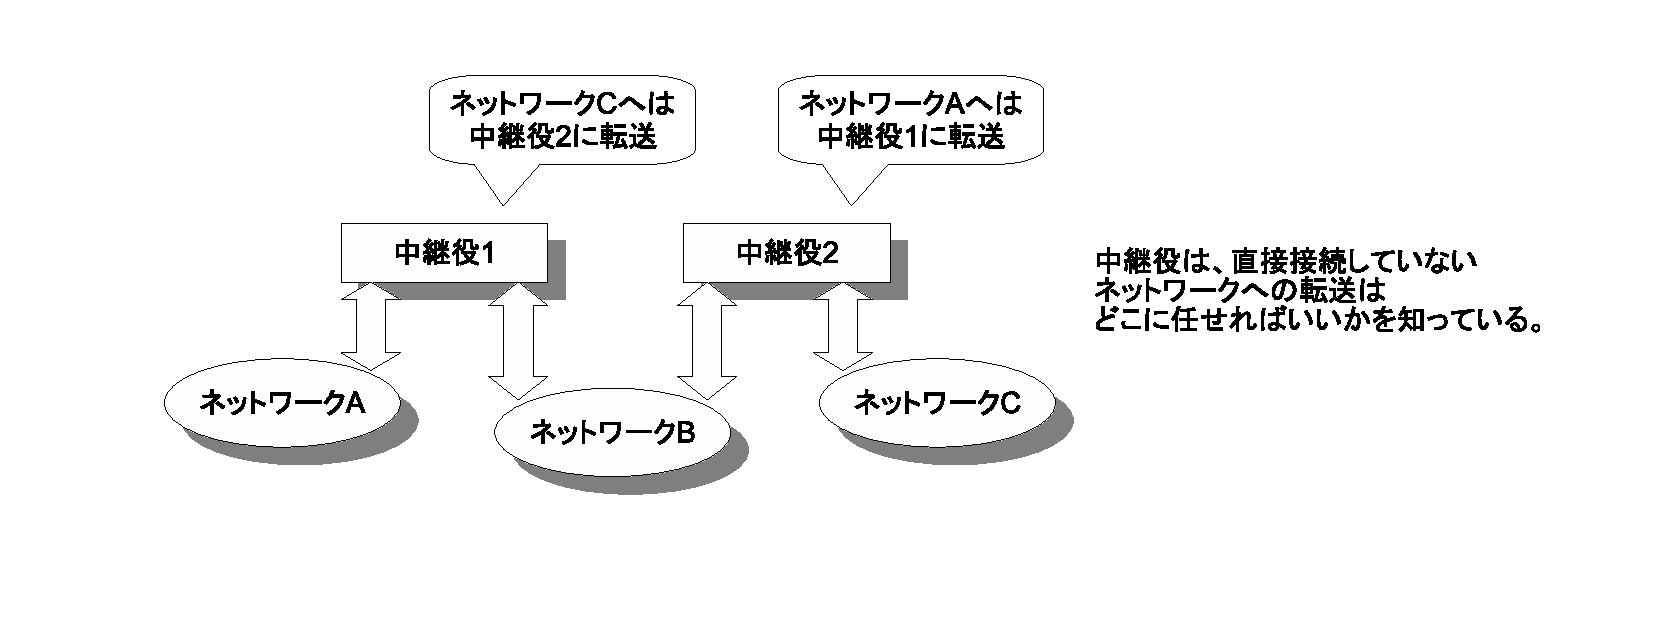
\includegraphics[width=12cm,clip]{draw/ip_basic3.eps}
	\caption{三つ以上のネットワークを結ぶ}
	\label{fig:ip_basic3}
\end{figure}

\subsection{もっとたくさんのネットワークが接続されている場合}

今度は、もっとたくさんのネットワークが接続されている場合について考えてみよう。
中継役は、自分が接続されているネットワークには自分で通信を中継する。また、自分が接続されていないネットワークが宛先であり、他のネットワークへの中継役と接続されていれば、その中継役に中継してもらう。

では、世界のどこかには存在するけれど、どこに存在するか知らない宛先と通信したいときはどうするか。中継役は、自分が知らない宛先への中継を丸投げする、別の中継先というのを知っている。
自分が知らない宛先への通信は、この中継先に丸投げする。

一見いい加減に思える方法であるが、インターネットの通信はこれで成り立っている。中継を繰り返すうちに、宛先へ向かう中継役を知っている中継役にいきつき、それを繰り返して、目的の宛先にたどり着くわけだ。いわばバケツリレーである。だが、廻されたバケツは自分の分かる範囲で適切と思われる宛先に渡す、という紳士協定に、すべての中継役は従っている。

\begin{figure}[htbp]
	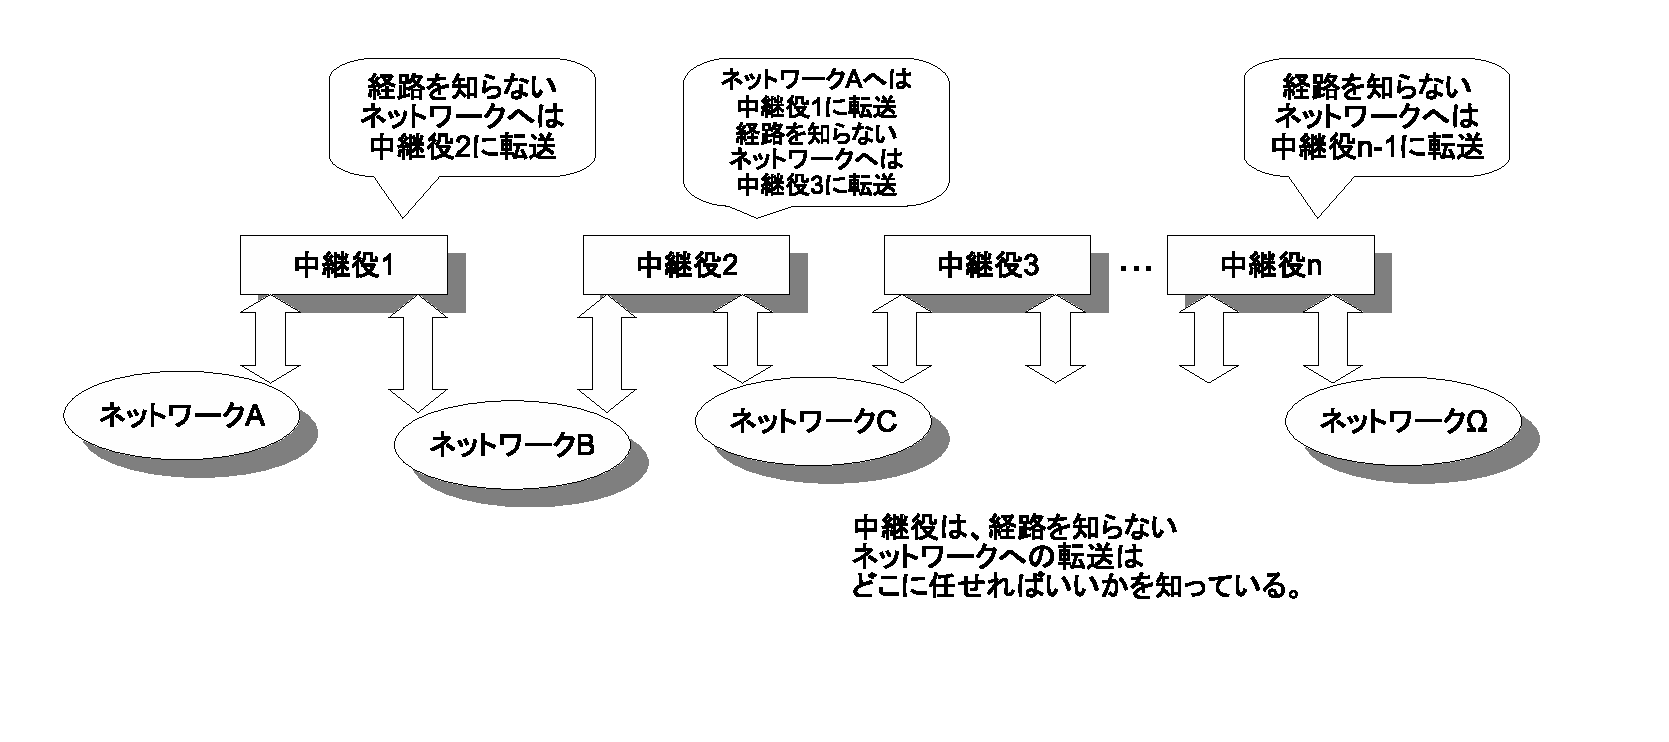
\includegraphics[width=12cm,clip]{draw/ip_basic4.eps}
	\caption{もっとたくさんのネットワークを結ぶ}
	\label{fig:ip_basic4}
\end{figure}

\subsection{ルータ}
ここまで中継役という名前で説明してきた機器が、現在ルータと呼ばれるものである。ルータは、届いた通信を、同じネットワークに接続されたホストを含む宛先に適切に中継するための機器である。

ネットワーク間の中継専用の機器であるルータは、1990年代半ばにCisco Networksがはじめて発売した。それ以前は、PCやワークステーションにネットワークインタフェイスを複数取り付け、中継専用に使用することが多かった。

\subsection{パケットとデータグラム}

ルータの通信は、ひとかたまりのデータを送り合う形で行われる。このひとかたまりのデータを、パケット、もしくはデータグラムと呼ぶ。パケット(Packet)は小包、データグラム(Datagram)は、データと電報(Telegram)の複合語である。

パケットには宛先が書かれている。ルータは、宛先情報を参照して、どこにパケットを転送するか決定する。

\subsection{デフォルトルートとルーティング}

ここまで、どこにあるかわからない宛先と通信するときに使う中継先となるルータを、デフォルトルートと呼んでいる。デフォルトルートには、同じネットワークに宛先がなく、宛先に接続されているルータがどこにあるかわからない場合に、とりあえず中継してもらうルータである。
あるネットワークのルータは、宛先が自分の接続されたネットワークでないパケットのうち、つぎにどのルータに転送すれば良いかわからないパケットを、自分のデフォルトルートに転送する。

ルータが一つだけ接続されているネットワークでは、そのルータが必ずデフォルトルートとなる。そのネットワークに接続されたホストは、そのルータをデフォルトルートとして設定することで、外部のネットワークとの通信が可能となる。

また、デフォルトルート以外のルータがあるときに、どのネットワークのホストと通信するときはどのルータに中継してもらう、という情報を、ルーティング情報やルーティングテーブルと呼ぶ。また、ルーティング情報に従って中継するルータを選択することを、ルーティングと呼ぶ。デフォルトルートとの通信も、「知らない宛先」に対するルーティング情報に従ったルーティングである。


\subsection{Tier1とフルルート}

\begin{figure}[htbp]
	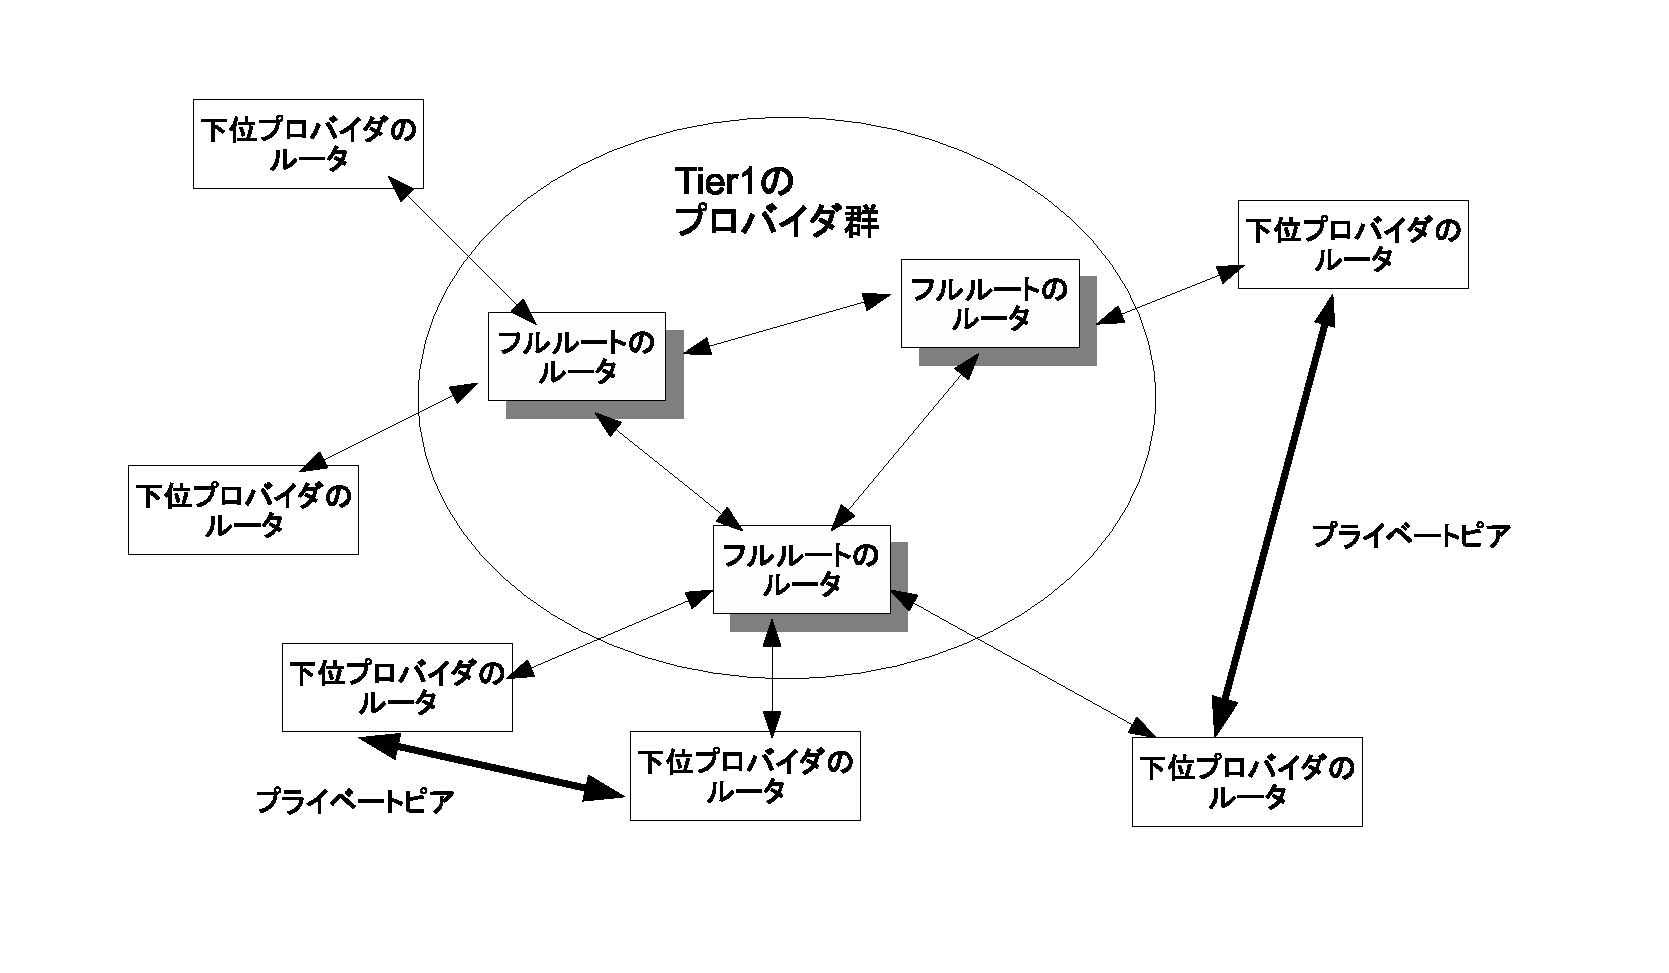
\includegraphics[width=12cm,clip]{draw/tier1.eps}
	\caption{Tier1プロバイダとプライベートピア}
	\label{fig:tier1}
\end{figure}


インターネットの通信とは、ここまで説明したバケツリレーを世界規模にしたものである。\footnote{CLANNADで、ことみのテディベアのエピソードを見ながら、インターネットプロトコルのパケットと同じだと思ったのは筆者だけではないであろう。}インターネットでは、ネットワーク毎に、デフォルトルートが存在する。
そして、インターネットの全てのネットワークからのパケットが届けられるルータは、全世界で25万ある経路について、次はどこに転送すればいいかを全て記憶している。

この全ての経路を、フルルートと呼ぶ。そして、フルルートを記録しているルータを管理するインターネットサービスプロバイダを、Tier1プロバイダと呼ぶ。
Tier1は、インターネットで一番多くの経路情報が集まる場所であり、宛先のわからないすべてのパケットが一度は送られる。Tier1のプロバイダを経由すれば、インターネットのどこにでもパケットを送ることができる。

\subsection{インターネットの構造}

インターネットの構造において、Iier1は、最上位のプロバイダになる。Tier1のプロバイダに、下位のプロバイダのネットワークが接続され、そのネットワークに、更に下位のプロバイダが接続される。このように、いくつものネットワークを相互に接続して、最終的にエンドユーザのネットワークに至る。
エンドユーザのネットワークは、そのネットワークに接続された下位のネットワークがない。インターネットの末端にあたる。

インターネットの構造は、Tier1によるネットワークを中心として、そのネットワークを相互接続されたネットワークが何重にも取り囲んでいる。その一番外側に、エンドユーザのネットワークが存在する。

\subsection{プライベートピア}

Tier1以外のプロバイダの間で、プライベートピアと呼ばれる経路が設定されていることがある。
これは、Tier1のプロバイダを介さずにその下位のプロバイダ同士でパケットを交換するための、専用線を使用した経路である。

プライベートピアを敷設する理由は、上位プロバイダと野接続料金の削減がある。プロバイダAとプロバイダBのネットワークの間にプライベートピアを設定すれば、この『プロバイダ間の通信はTier1を通す必要が無い。それによって、パケットが上位のに行くための時間を削減できる。
また、上位のプロバイダと野接続料金を削減する効果もある。データ通信の回線は、パケットの転送数で料金が決まる契約となっていることがある。そのため、撚りやすい回線でプライベートピアを構成すれば、その分の回線費用を抑えることができる。



\subsection{ダイナミックルーティング}

あるパケットが宛先に届くときの経路は、毎回同じであるとは限らない。あるパケットと、その次に届いたパケットは、それぞれ全く別の経路を通って届いた可能性がある。

これは、その時点でのネットワークの状況で経路を決める、ダイナミックルーティングを行うルータが経路の途中にあるためである。ダイナミックルーティングは経路に障害が発生していたり、負荷が高かったりするときに、転送する先のルータを変更する。そのため、パケットの経路は、パケットごとに異なる可能性がある。

\subsection{パケットの到着順}
パケットは、一つ一つの経路が異なる可能性がある。そして、経路が違えば送信した順番を崩して宛先に届くこともある。

インターネットプロトコル層は、パケットが送信順に宛先に届くことを保証しない。もしそれが必要なら、トランスポート層やアプリケーション層でそれを担保するのがインターネットプロトコルスイートの考え方である。
インターネットプロトコル層が担当するのは、パケットを宛先により近そうなルータに向けて転送することだけである。


\subsection{なぜ世界はひとつのイーサネットではないのか}

ここまでの説明で、ルータでなくても、世界中イーサネットにしてブリッジで繋げばいいのではないか、そう思う読者諸兄がいるかもしれない。ここで、ルータとブリッジの違いに触れておこう。

ルータは、適切なルーティングを行うことで、いくつものルータを介して接続された「遠隔」かつ「複数」のネットワークうに対して通信を行うことができる。ネットワークコミュニケーション層よりも広い範囲で、ネットワークを越えた相互通信を行うためにインターネットプロトコル層が存在し、そして、そのための機器としてルータが存在するわけだ。
また、異なる規格のネットワークの間でも、パケットを中継することができる。たとえば、離れた二点間の通信に向くPPP接続によるネットワークと、ある範囲に多数のホストがあるときに向く、イーサネットによるネットワークとの間で、パケットによる通信ができる。

ブリッジは直接接続された衝突ドメイン間での、フレームの転送をを可能とするだけである。
また、規格の異なるネットワークコミュニケーション層のプロトコルを変換氏、相互通信を行うことはできない。
ブリッジで接続されたネットワークは、ネットワークコミュニケーション層での同じネットワークとなり、物理的な大きさの限度が存在する。



\subsection{インターネットプロトコルのアイディア}

ここまで説明したことが、大まかなインターネットプロトコルのアイディアである。初期のTCPとIPの機能は分離していなかった。
ネットワーク間でデータを転送する機能をインターネットプロトコルとして分離させたのは、TCPv3とIPv3という、TCP/IPのいわばバージョン3からである。

その後、IPのバージョンが4となる。このIPv4が、現在インターネットで使用されるアドレスと、それによる転送ルールなどの体系として、現在に至るまで30年以上使用されている。
現在は、IPv4と、その後継となるIPバージョン6、つまりIPv6とが併用されている。

\subsection{コネクションレス通信}

先に説明したように、インターネットプロトコル層のデータの単位を、パケットもしくはデータグラムという。宛先情報であるヘッダと、データから構成されているのが、小包や電報とにていることから付けられた名前である。
パケットとは、電話のように、端から端まで物理的に回線を接続するコネクション型の通信と対比しての呼び方である。両端まで接続された回線をデータが流れるときは、「宛先」情報はいらない。なぜなら、送信する側の反対側が必ず宛先であるからだ。

だが、データに宛先情報を付加し、途中で宛先情報を参照して適切な宛先に転送する仕組みがあれば、たとえ送信側から受信側まで一本の経路が繋がっていなくても、そのデータはいつか宛先に辿り着くだろう。これが、、パケットの考え方である。ここまでの説明の言葉を使えば、宛先の書いてあるバケツということになる。
そのため、パケットを使う通信は、コネクション型通信に対比して、コネクションレス通信と呼ぶ。

\section{そもそもインターネットとは何か}

インターネットという言葉とは、インターネットプロトコルで接続されたネットワークのによって構成されるネットワーク事指す。
ここで気をつけるべきは、インターネットプロトコル使用して相互接続される複数のネットワークなのでインターネットと呼ばれる、ということだ。インターネットで使用するプロトコルだから インターネットプロトコルなのでは内。

\subsection{internnetとInternetの違い}

「インターネット」と読む語には、一般名詞としてのinternetと、固有名詞としてのInternetの二つが存在する。この二つの言葉には、それぞれどんな意味があるのであろうか。簡単にではあるが、辞書を引いてみることにしよう。

\begin{description}
\item[internet]単一の論理ネットワークを構築するために、共通のプロトコルで接続された複数の物理ネットワーク
\item[Internet]小文字で始まるinternetが相互接続された世界規模のネットワーク\footnote{定冠詞をつけてthe Netと表記する場合もある。}
\end{description}

一般名詞のinternetは、この章で説明するインターネットプロトコルによって相互接続されたネットワークの集合遺体を指す。辞書的な意味に従えば、二つのネットワークコミュニケーション層をインターネットプロトコルで相互接続すれば、それはもうinternetである。

固有名詞のInternetは、ARPAnetと呼ばれる、1969年に、アメリカで4つの大学を接続することから始まったネットワークの相互接続実験に端を発するネットワークである。
ARPAnetは、もともとTcP/IPを使用していなかった。だが、1980年代初頭にARPAnetのプロトコルがTCP/IPに置き換えられている。

\section{インターネットプロトコル層}

ここまで説明したように、複数のネットワークコミュニケーション層を相互接続するためのレイヤーを、インターネットプロトコル層と呼んでいる。
そして、インターネットプロトコルとは、インターネットプロトコル層で用いる通信規約である。
では、ここから、インターネットプロトコルについて、もう少し立ち入って説明していくことにしよう。

インターネットプロトコルには、おおまかに、以下のような役目がある。

\begin{itemize}
\item ネットワークとホストを識別するための、インターネットプロトコルアドレスを定義する 
\item インターネットプロトコル層でのデータの単位であるデータグラムを定義する 
\end{itemize}

固有名詞のInternetは、ARPAnetと呼ばれる、1969年に、アメリカで4つの大学を接続することから始まったネットワークの相互接続実験に端を発する。通常の教科書であればARPAnetのはじまりからTCP/IPの導入。発展的解消への歴史を説明すべきところであろう。だが、本書では、ARPAnetはTCP/IPに依って構築されたのでなく、1980年代初頭にARPAnetのプロトコルがTCP/IPに置き換えられた、という卵と鶏のどちらが先かの説明に留めておくことにする。\footnote{ARPAnetの歴史に興味があれば、参考文献に挙げた書籍を参照していただきたい。}




\section{インターネットプロトコル層}

ここまで説明したように、複数のネットワークコミュニケーション層、つまり、物理ネットワークを相互接続するための層を、インターネットプロトコル層と呼んでいる。そして、インターネットプロトコルとは、インターネットプロトコル層で用いる通信規約である。では、ここから、インターネットプロトコルについて、もう少し立ち入って説明していくことにしよう。

インターネットプロトコルには、おおまかに、以下のような役目がある。本章では、この役目の一つ一つについて、説明を行っていく。

\begin{itemize}
\item ネットワークとホストを識別するための、インターネットプロトコルアドレスを定義する 
\item インターネットプロトコル層でのデータの単位であるパケットを定義する 
\item ネットワークコミュニケーション層とトランスポート層を仲立ちする 
\item ルーティングする
\item パケットにするには大きすぎるデータがきたとき、分割(フラグメント)する
\end{itemize}

\subsection{IPv4と」IPv6}
概論において簡単な説明を行ったが、現在、インターネットプロトコルにはバージョン4とバージョン6という二つのバージョンが存在する。

もともと、インターネットプロトコルスイートで用いられていたインターネットプロトコル層は、バージョン4である。
だが、90年代に、バージョン4では、各ホストやネットワークを一意に区別するのに用いる番号であるIPアドレスが足りなくなることが予想された。
そのため、取り得るIPアドレスの数を増やすことを第一の目的として策定されたのが、インターネットプロトコルのバージョン6(IPv6)である。
IPv6では、アドレス数を増やす以外の拡張、変更も多く行われている。

本書第6版発行現在(2018年秋)はその過渡期であり、IPv4が主に使われている中、IPv6もユーザに意識させないまま普及が進んでいる。
本書では、インターネットプロトコルのバージョン4をIPv4、バージョン6をIPv6と表記する。

\subsection{デュアルスタック}

IPv4とIPv6が併用されているということは、ふたつの「インターネットプロトコル」が併用されているということである。

インターネットプロトコルスイートにおいて、インターネットプロトコル層の部分におさまるなにかが、二つ存在するということだ。では、この二つはどのような位置関係にあるのだろうか。

インターネットプロトコルスイートの菱餅重ねのなかにIPv4とIPv6をいれななおしてみると、図\ref{fig:dualstack}のように、二つのプロトコルが隣り合った位置に配置される。

トランスポート層は、このどちらの「インターネットプロトコル」も使うことができる。また、どちらのインターネットプロトコル層も、同様にトランスポート層にサービスをする。そして、どちらのインターネットプロトコル層も、ネットワークコミュニケーション層からサービスを受ける。

つまり、実際のネットワークでは、IPv4とIPv6を同時に使うことができるということだ。このことを、インターネットプロトコル層のスタックが二つある、という意味で、デュアルスタックとよんでいる。

\subsection{デュアルスタックの優先順}

\begin{figure}[htbp]
	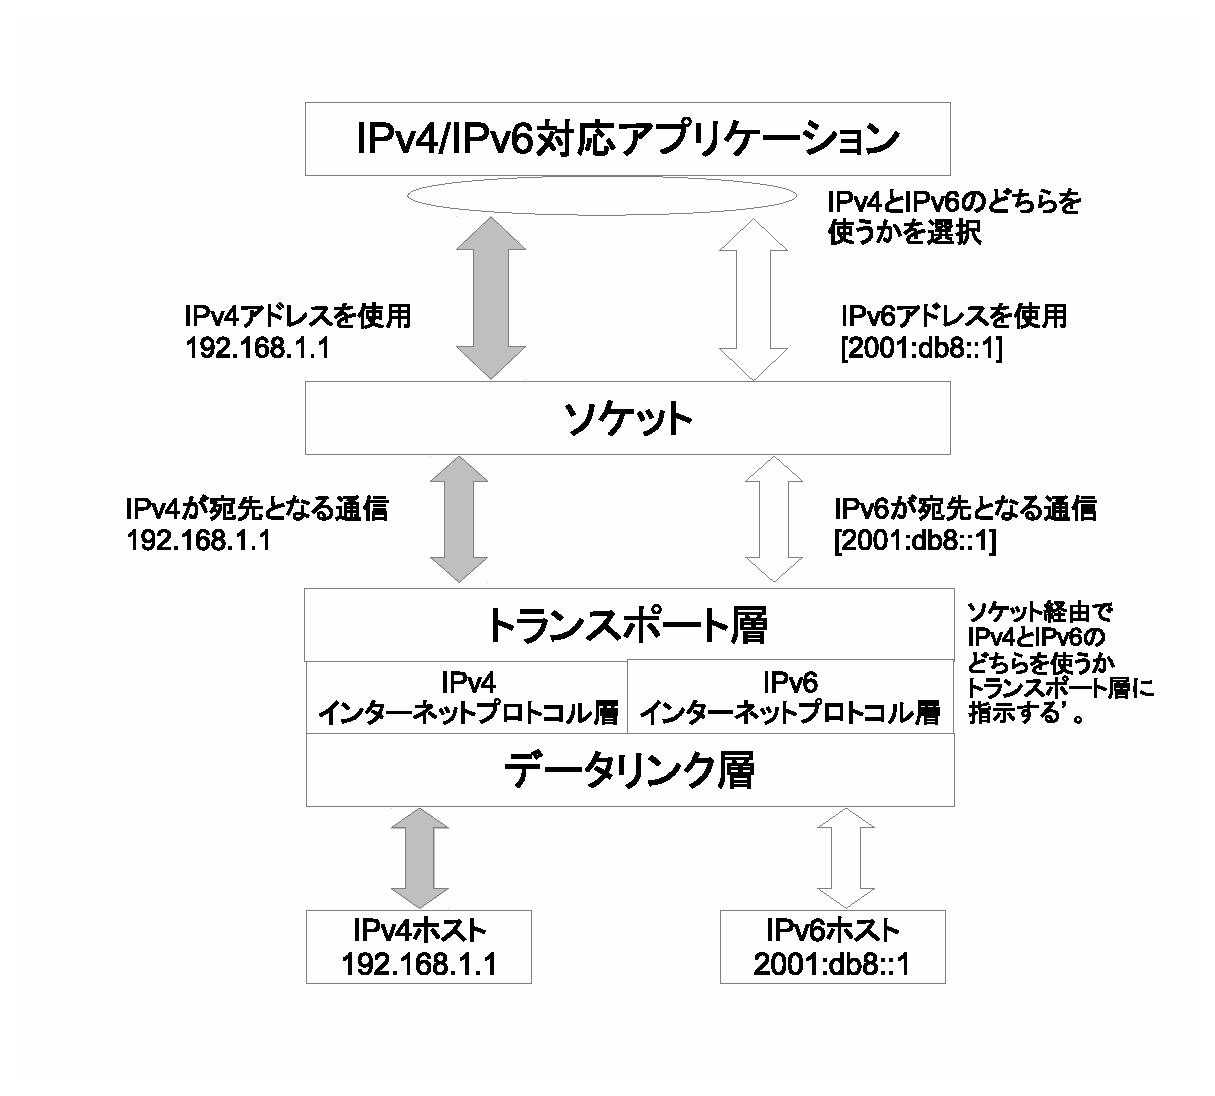
\includegraphics[width=12cm,clip]{draw/doublebind.eps}
	\caption{デュアルスタック}
	\label{fig:dualstack}
\end{figure}

デュアルスタックの環境かつ、IPv4とIPv6のどちらでも、同じホストに到達できる場合、どちらのインターネットプロトコル層を使うのだろうか。
デュアルスタック環境では、まずIPv6によるアクセスが可能なら、IPv6でのアクセスを試みることになっている。IPv6での接続が規定の時間内に終了しない場合、あらためてIPv4でのアクセスを試みる。

実は、この選択を行うのはアプリケーション層である。実装上、アプリケーションがソケットを開くとき、アドレスファミリを選択することで、IPv4とIPv6のどチラを使うか、どちらから使うかを選択する。
IPv4のスタックはIPv4のスタックとしか通信できない。IPv6も、IPv6としか通信できない。インターネットプロトコル層には、どちらのスタックを使うべきかの判断をする自動判別のロジックは持っていない。


\section{インターネットプロトコルアドレス}

インターネットプロトコルという言葉で最初に思いつくものはなにであろうか。それはおそらく、インターネットプロトコルアドレス(Internet Protocol Address、以降IPアドレス)ではないだろうか。

IPアドレスとはその名の通り、インターネットプロトコルで接続されるネットワークにおいて、ホストとネットワークを識別するためにユニークにつけられる番号であり、これをアドレス\footnote{後で説明するように数字の列であるが、建物の号室表示までついた文字通りの住所と考えてよい。}と呼び表す。

\subsection{IPv4アドレスとIPv6アドレス}

先だって、インターネットプロトコル層として、二つのバージョンが併用されているという話をした。つまりIPアドレスも、それぞれのバージョンに対応したものが存在する。

IPアドレスは、最初は、IPv4の形式が実用化された。4組の数字をドットで区切った、192.168.1.1というような形式のアドレスである。
このIPv4でのIPアドレスは、32bitのビット列によって表される。数字表記は、人間が理解しやすいようにするために、先頭から8bitごとに区切って、それを十進数であらわしたものとなる。

IPv4アドレスは、0.0.0.0から255.255.255.255までのアドレスを取り得る。
では、IPv4アドレスはいくつ存在すのだろうか。IPv4アドレスは、32bit長なので、$2^{32}$個存在することができる。これを書き下すと4294967296個で、約43億個である。


一方のIPv6のアドレスは、128bitのビット列によって表される。これは、$2^{128}$個である。これを書き下すと、
340282366920938463463374607431768211456個
という膨大な数となる。

IPアドレスの総数と表記法は、IPv4とIPv6とで、一番目に付きやすいので、そえrを比較してみることにする。
IPアドレスは、数字がドットで区切られてよっつ並んでいるだけに見える。だが、IPアドレスは単純な通し番号としてつけられているわけではない。

IPv4アドレスは、32bitのビット列で表される。それを分かりやすくするために、8ビット毎に区切って10進数にして、ドット区切りで記述する。\footnote{IPv6では、128bitを16bitづつコロン:で区切り、その区切られたものを16進表記する。} おそらく、192.168.0.1というような記述をされているIPアドレスを目にしたこともあるであろう。アドレスの種類としては、特別な意味があるので割り当てないものなども含めて、0.0.0.0から255.255.255.255まで$2^{32}$通りの記述が可能である。

一方のIPv6は、128bitを16bitづつコロンで区切り、その区切られたものを16進表記する。4桁の16進数が8個並ぶものとなる。たとえば、2001:0db8:0000:0000:0000:0000:0000:0001というような表記となる。そのため、IPv6のアドレスには、省略記法が定められている。その省略記法に従えば、先のアドレスは2001:0db8::1と記述することができる。
この省略記法については、後ほど改めて説明する。



\subsection{IPv4アドレスは多いのか少ないのか}
IPv4のアドレスは、$2^{32}$個存在することができる。後述するように、特別な意味があって割り当てないアドレスも含めて、およそ43億個のアドレスである。果たして、このアドレスは多いのだろうか、それとも少ないのだろうか。

本書刊行の2018年10月現在、APNICからアジア太平洋地区に新たに割り当てられるIPアドレスはない。割り当てを受けたインターネットプロバイダが配布するものがあるだけである。なのはでもまどかでもなく、IPアドレス完売、である。一方アメリカのIPアドレスを管理するARINにはIPv4割り当てに余裕がある。そのため、アメリカのインターネットサービスはIPv6への対応が遅いという別の問題もある。

43億個のアドレスは、世界中にインターネット接続可能な機器が存在する現在、とても足りるわけがない数である。
とはいえ、TCP/IPの実用化が始まった時代には、十分に多かったことも事実である。何より、アドレスに4オクテット分も、貴重な通信時間を割いていたのだ。では、その当時、IPアドレスを持っていたホストが世界中でいかにに少なかったかを示すエピソードを披露しよう。

Unixには、/etc/hostsという、IPアドレスとホスト名の対応を書いた、一覧表のファイルがある。\footnote{Windowsにも該当するhostsファイルが存在する}、
これは、DNS開発以前に、ARPAnetに接続されていた全ホストの情報をFTPで配布していた名残である。このファイルは、当時のARPAnetに新しいホストが追加される毎に、FTPで新しいものが配布されていた。IPv4実用化の頃は、4億個というのが永遠に使い切ることがないと思えた、途方もないアドレス数であったことが伺えるエピソードである。

一方のIPv6のアドレス数$2^{128}$個は、いまのところ十分に多い数である。よく使われる例えとして、地球上の砂粒全てにIPアドレスを割り当てられるという表現がされることもある。\footnote{ひとつのネットワークに割り当て可能なホスト数だけでも、およそ$1.84*10^{19}$個という膨大な数となる。}

\subsection*{いもうとコラム IPsec}
インターネットプロトコル層での通信に、認証と暗号化のオプションを付加するセキュリティ関連の規格に、IPsecがあります。IPv4では後付けの機能でしたが、IPv6では必須となりました。

IPsecは、インターネットプロトコル層のペイロードに認証ヘッダを付けたり、暗号化したりします。そのため、トランスポート層以上で何を使っているのかにかかわらず利用できます。
IPsecについての詳細は、それだけで専門書も多く出ているので、そちらを参照してください。

